%last updated in April 2002 by Antje Endemann

\documentclass[runningheads]{llncs}
%In order to omit page numbers and running heads
%please use the following line instead of the first command line:
%\documentclass{llncs}.
%Furthermore change the line \pagestyle{headings} to
%\pagestyle{empty}.
\usepackage{graphicx}

\input{psfig.sty}

\begin{document}

\pagestyle{headings}
%In order to omit page numbers and running heads
%please change this line to
%\pagestyle{empty}
%and change the first command line too, see above.

\mainmatter

\title{Camera pose from face images}

\titlerunning{Camera pose from face images}

\maketitle

\begin{abstract}
Abstract
\dots
\end{abstract}

\section{Introduction}

\section{Motivation}
Facial appearance can change dramatically due to distance to the camera and perspective distortion.  See figure \ref{fig:fiducial_migration}

\begin{figure}[ht]
\begin{tabular}{ccc}
\includegraphics[width=.3\linewidth]{../resources/figures/extracted_fiducial_0006.png} &
\includegraphics[width=.3\linewidth]{../resources/figures/extracted_fiducial_0008.png} &
\includegraphics[width=.3\linewidth]{../resources/figures/extracted_fiducial_0001.png} \\
\includegraphics[width=.3\linewidth]{../resources/figures/extracted_fiducial_0002.png} &
\includegraphics[width=.3\linewidth]{../resources/figures/extracted_fiducial_0003.png} &
\includegraphics[width=.3\linewidth]{../resources/figures/extracted_fiducial_0004.png} \\
\includegraphics[width=.3\linewidth]{../resources/figures/extracted_fiducial_0005.png} &
\includegraphics[width=.3\linewidth]{../resources/figures/extracted_fiducial_0007.png} &
\includegraphics[width=.3\linewidth]{../resources/figures/fiducial_migration.png}
\end{tabular}
\caption{A face at different camera distances and focal length (zoom) along with the migration of fiducials (bottom right).}
\label{fig:fiducial_migration}
\end{figure}

\section{Data}
We use the GavaBDB\cite{moreno2004gavabdb} dataset.
\begin{figure}[ht]
\begin{tabular}{cc}
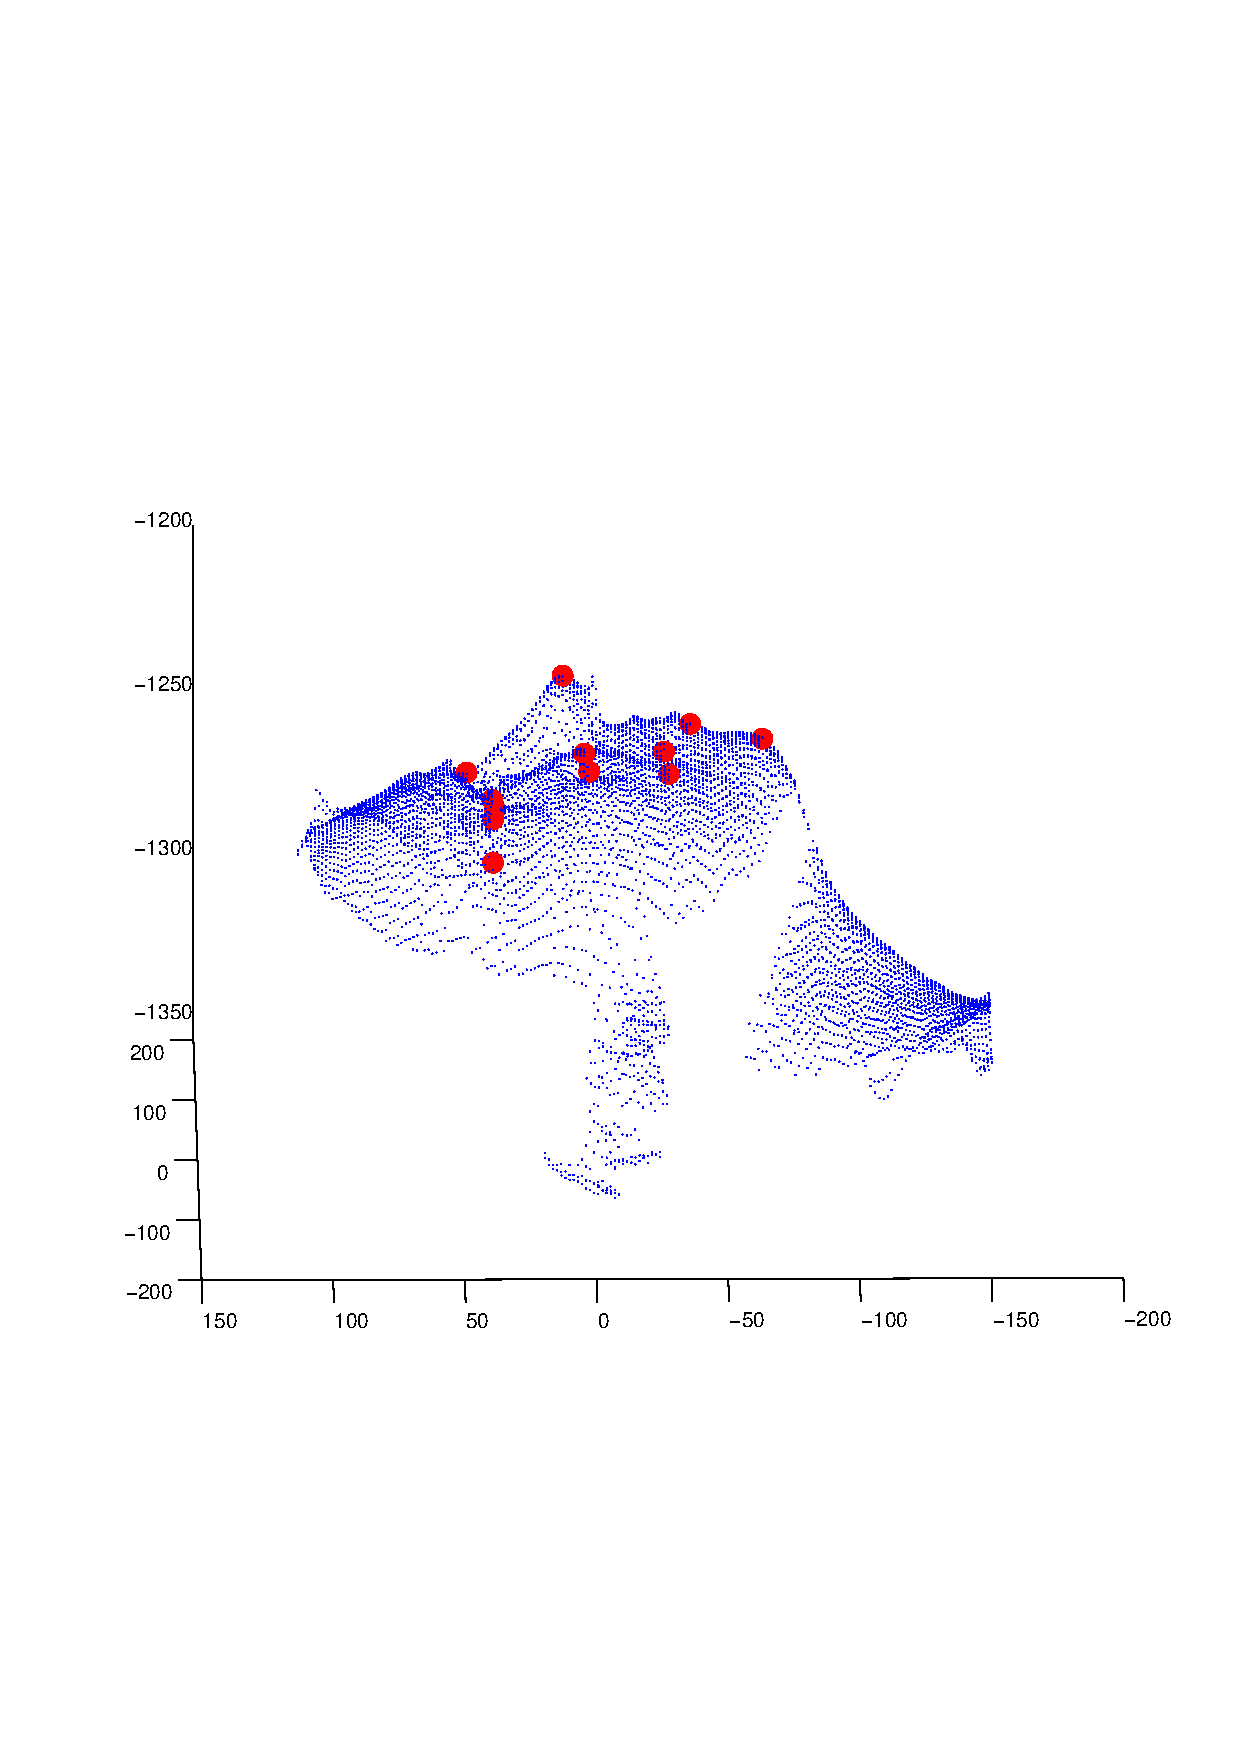
\includegraphics[width=.4\linewidth]{../resources/figures/face1.png} &
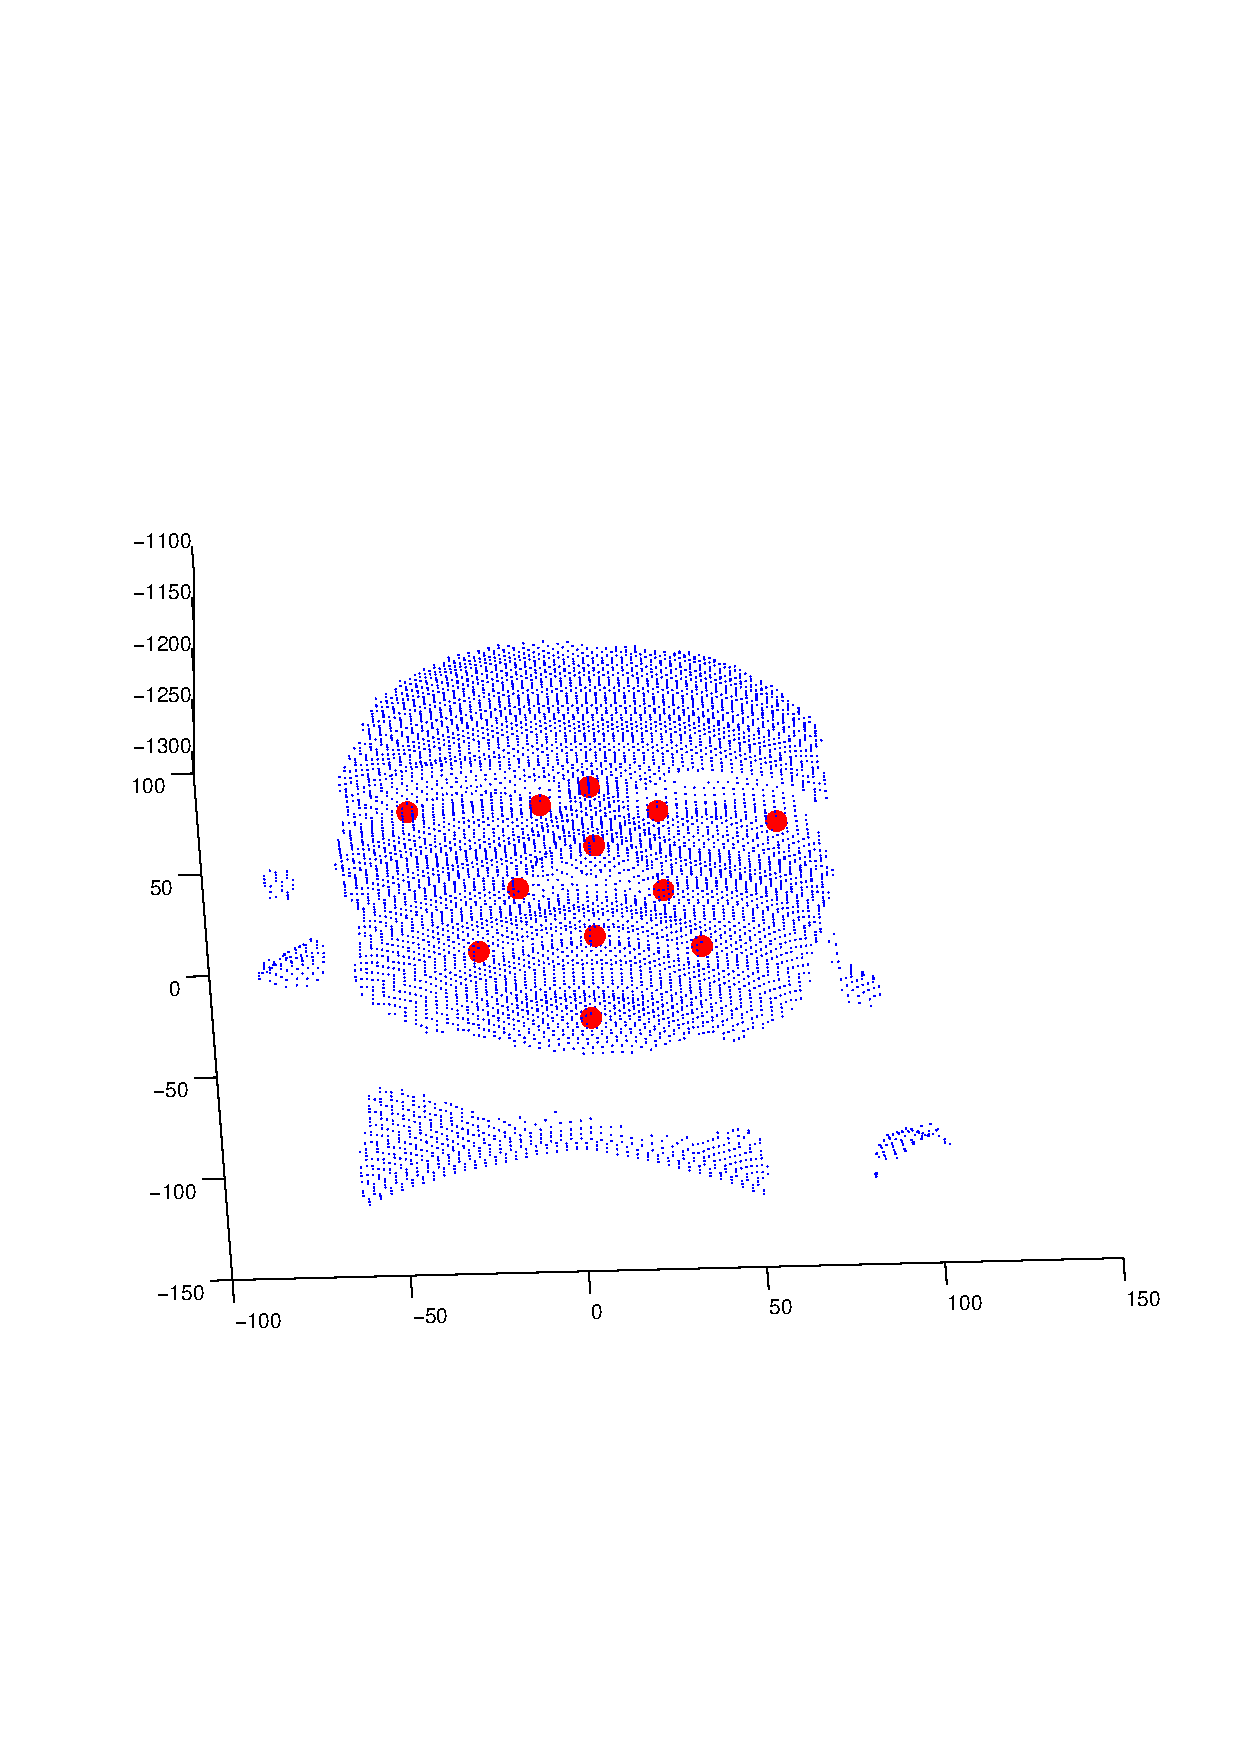
\includegraphics[width=.4\linewidth]{../resources/figures/face2.png} \\
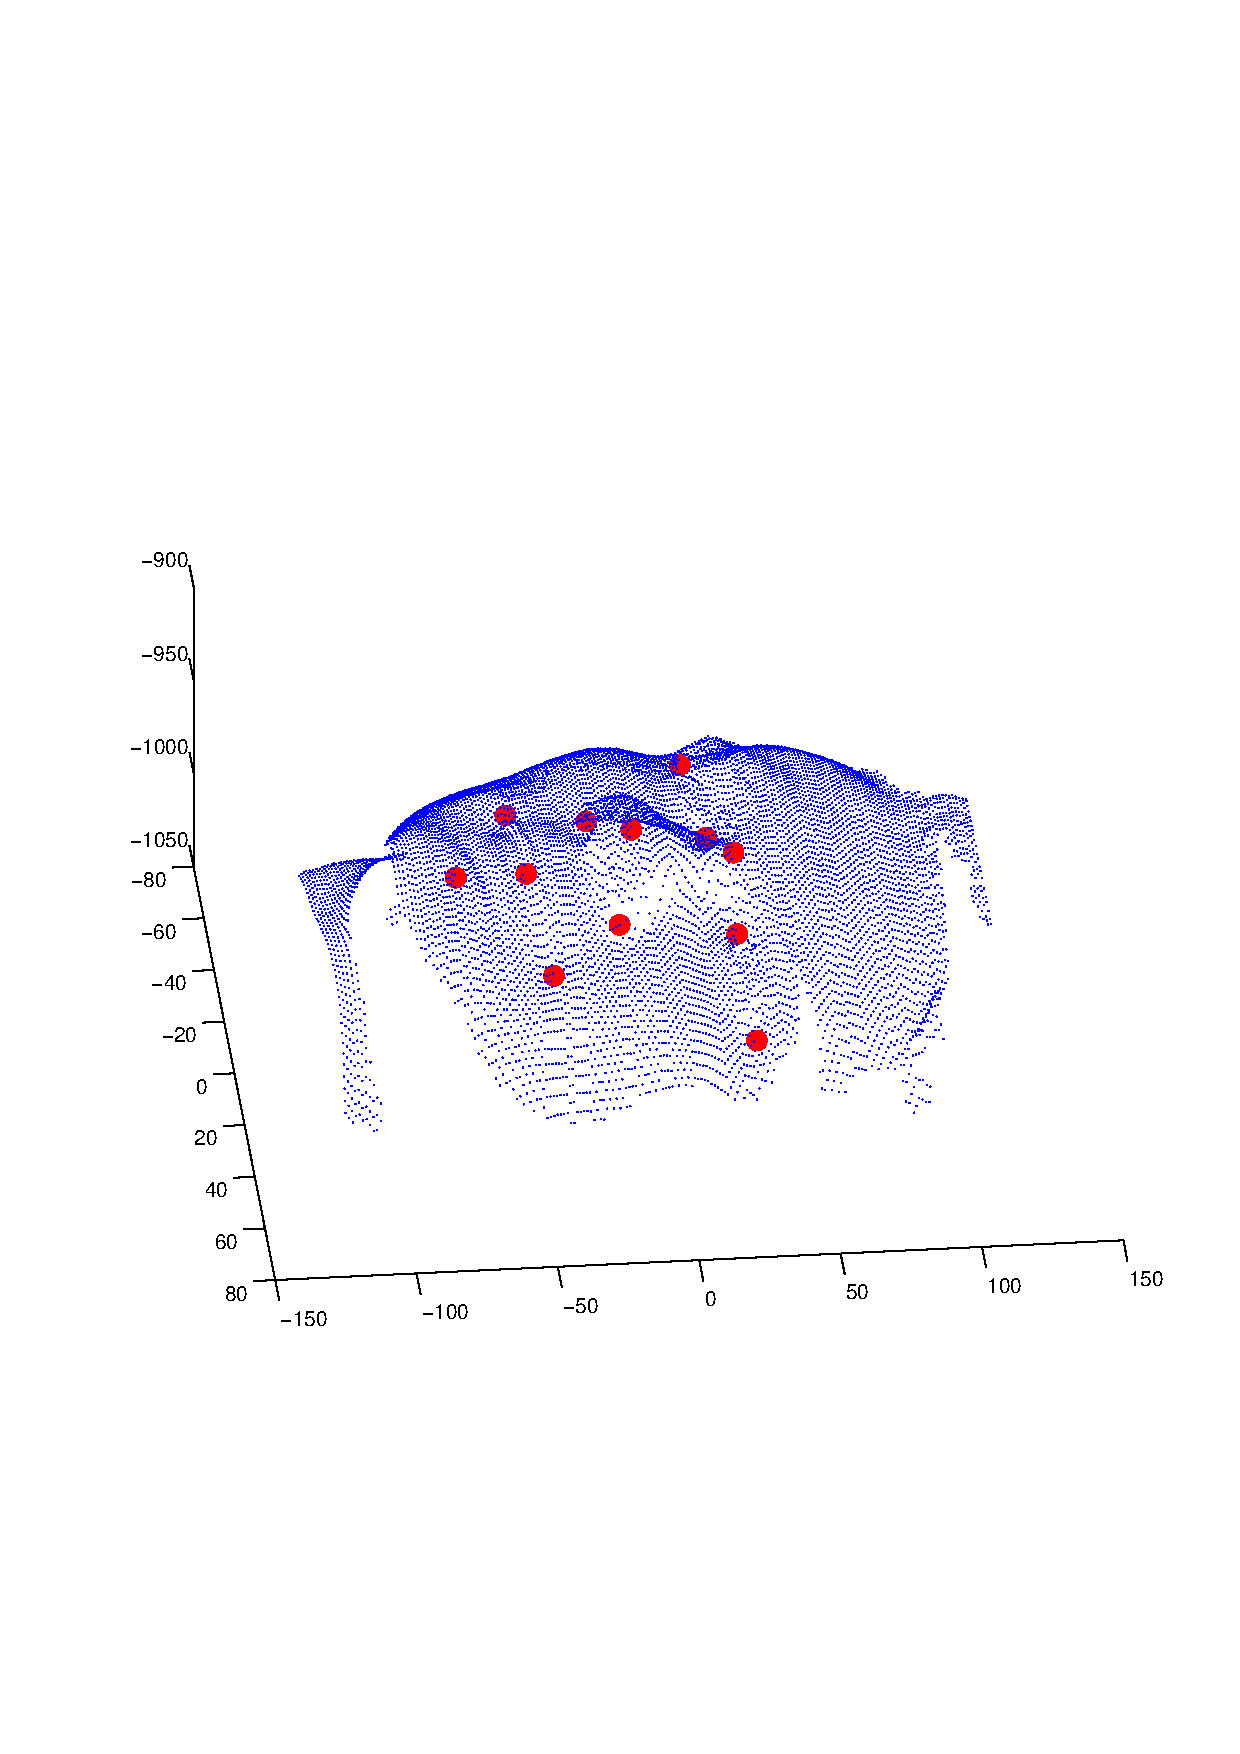
\includegraphics[width=.4\linewidth]{../resources/figures/face3.png} &
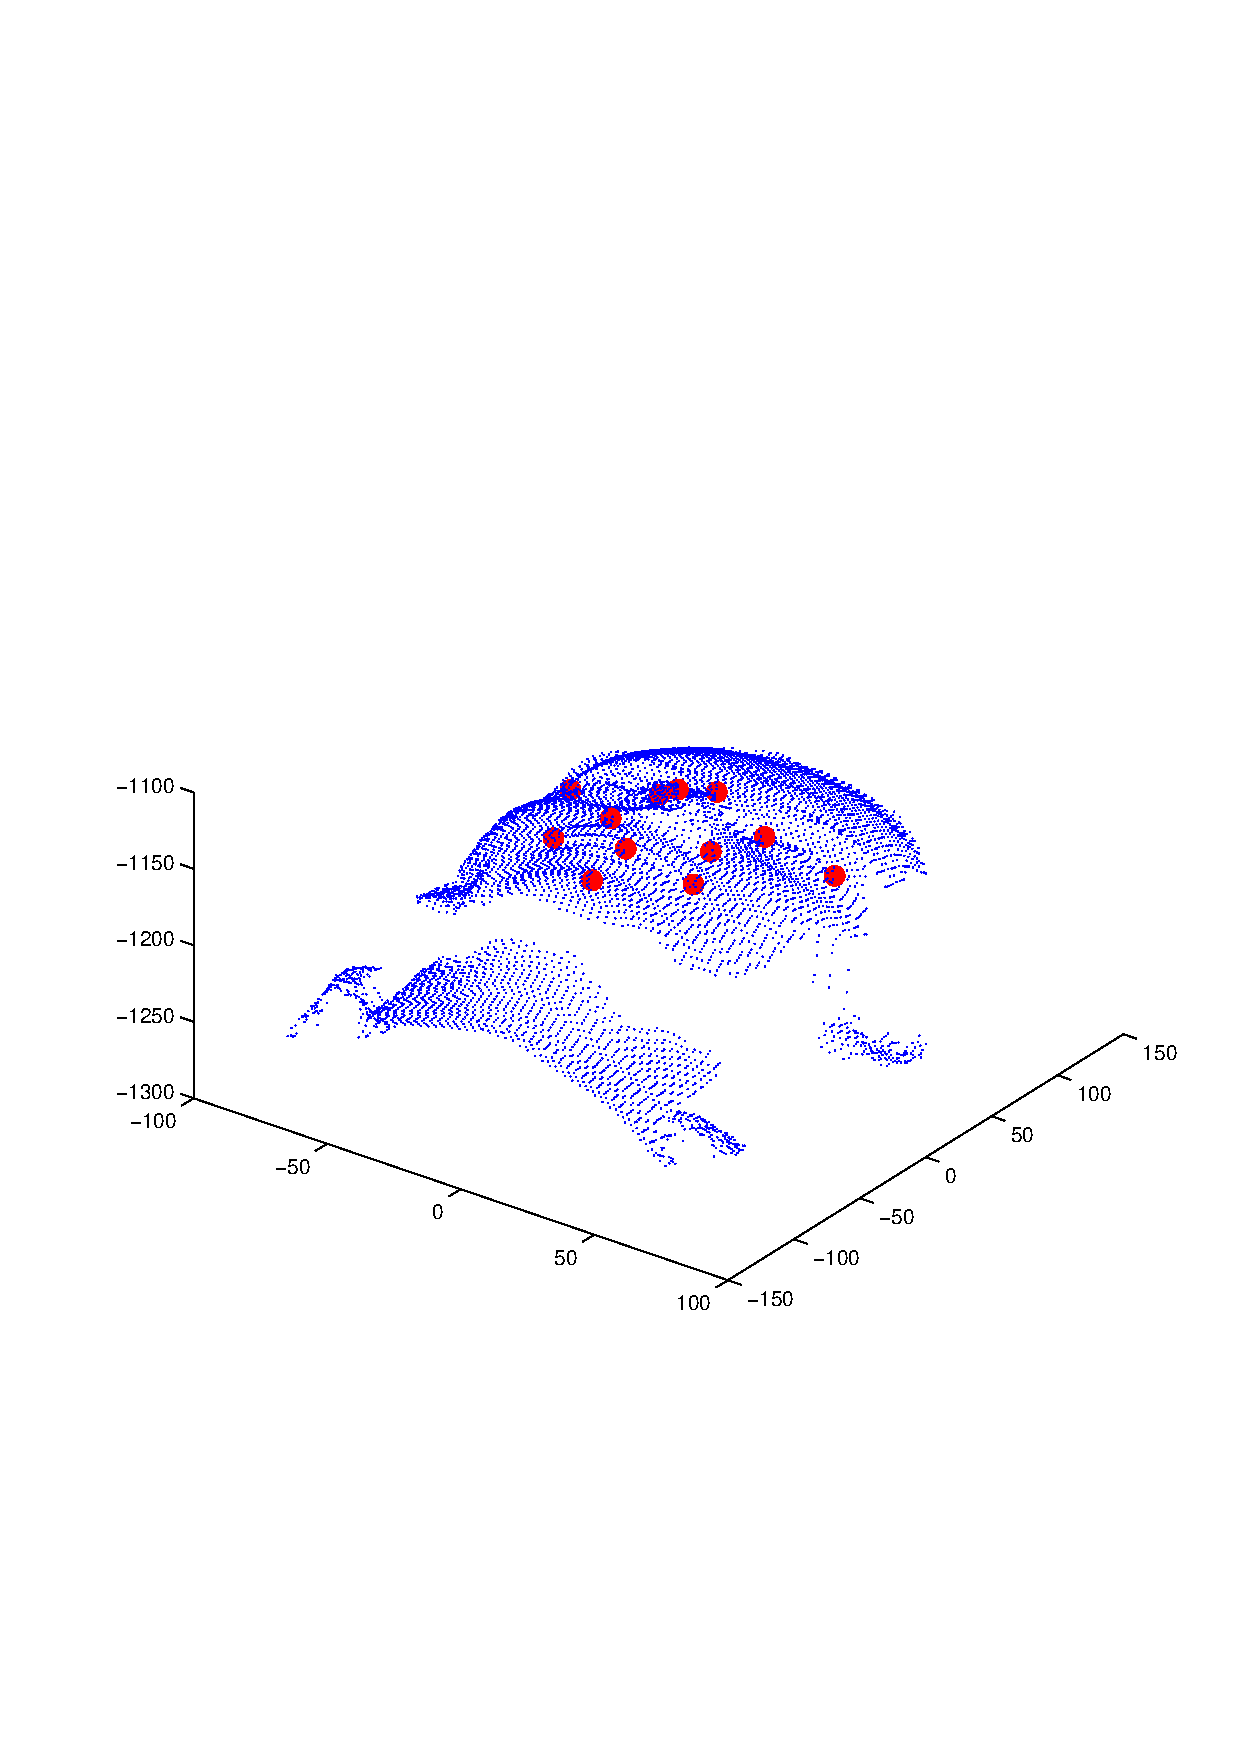
\includegraphics[width=.4\linewidth]{../resources/figures/face4.png}
\end{tabular}
\caption{Point clouds of four different individuals and different view angles.  Large red dots indicate fiducial locations.}
\end{figure}

\section{Camera pose estimation using EPnP}
Inspired by \cite{ohayon2006robust}.  We use Lepetit's EPnP \cite{lepetit2009epnp}.

\section{Results}

\begin{figure}[ht]
\begin{tabular}{cc}
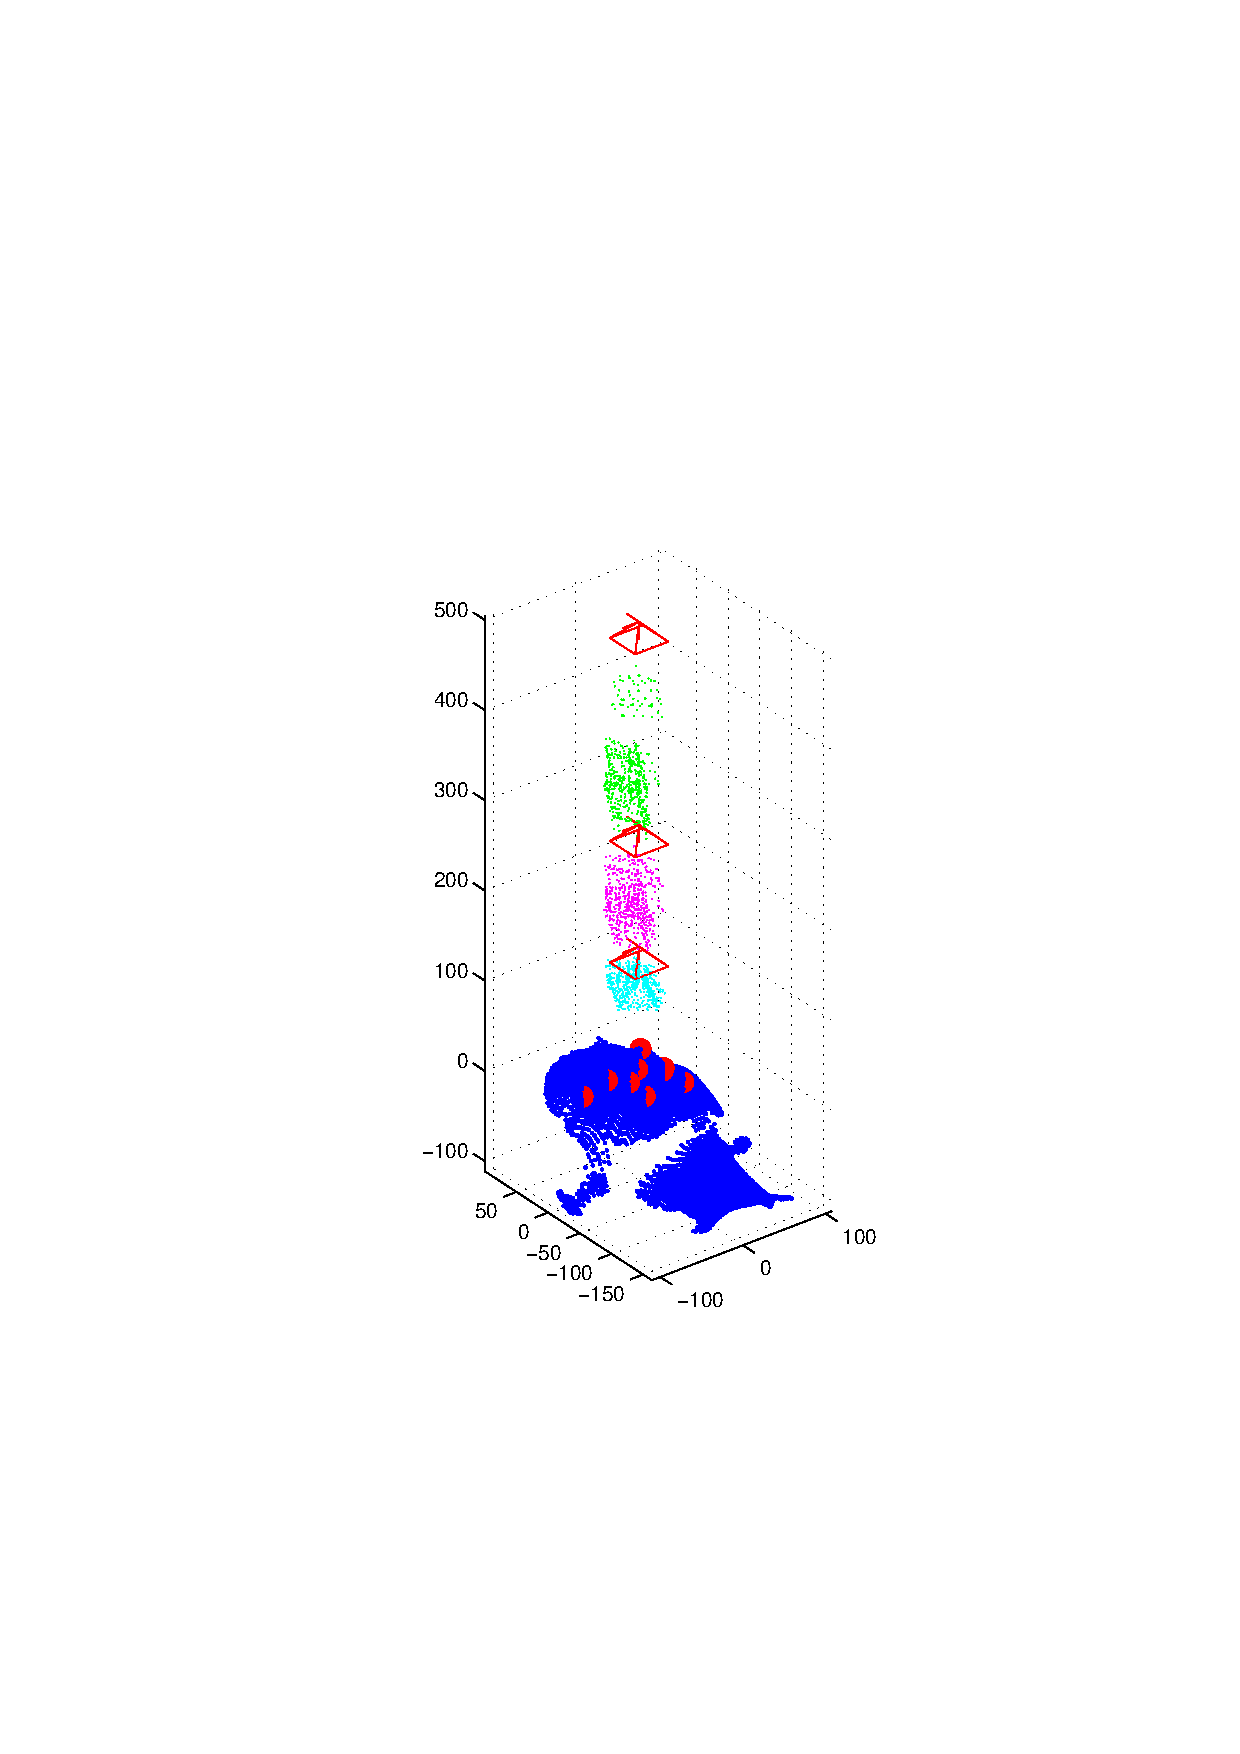
\includegraphics[width=.45\linewidth]{../resources/figures/cameraloc_frontal.png} &
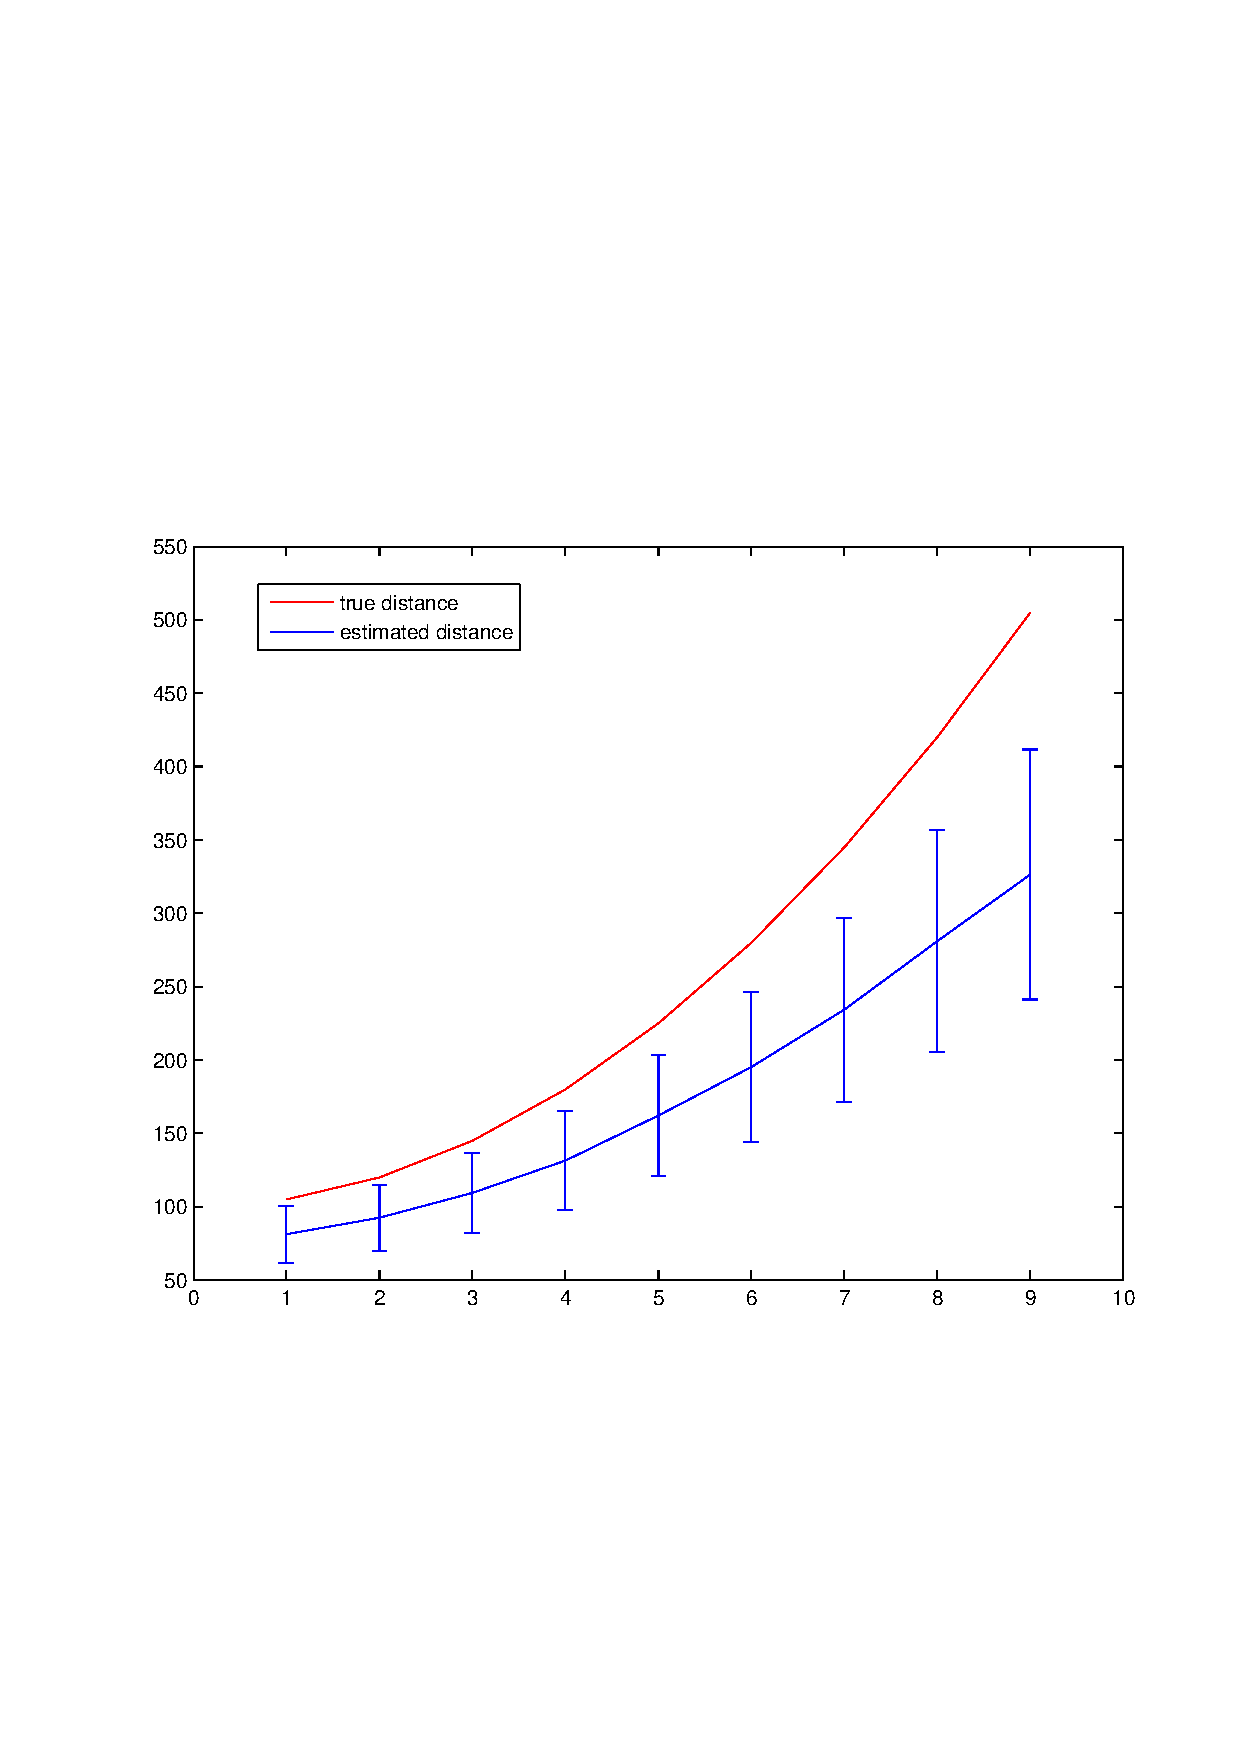
\includegraphics[width=.45\linewidth]{../resources/figures/errorbar_frontal.png} \\
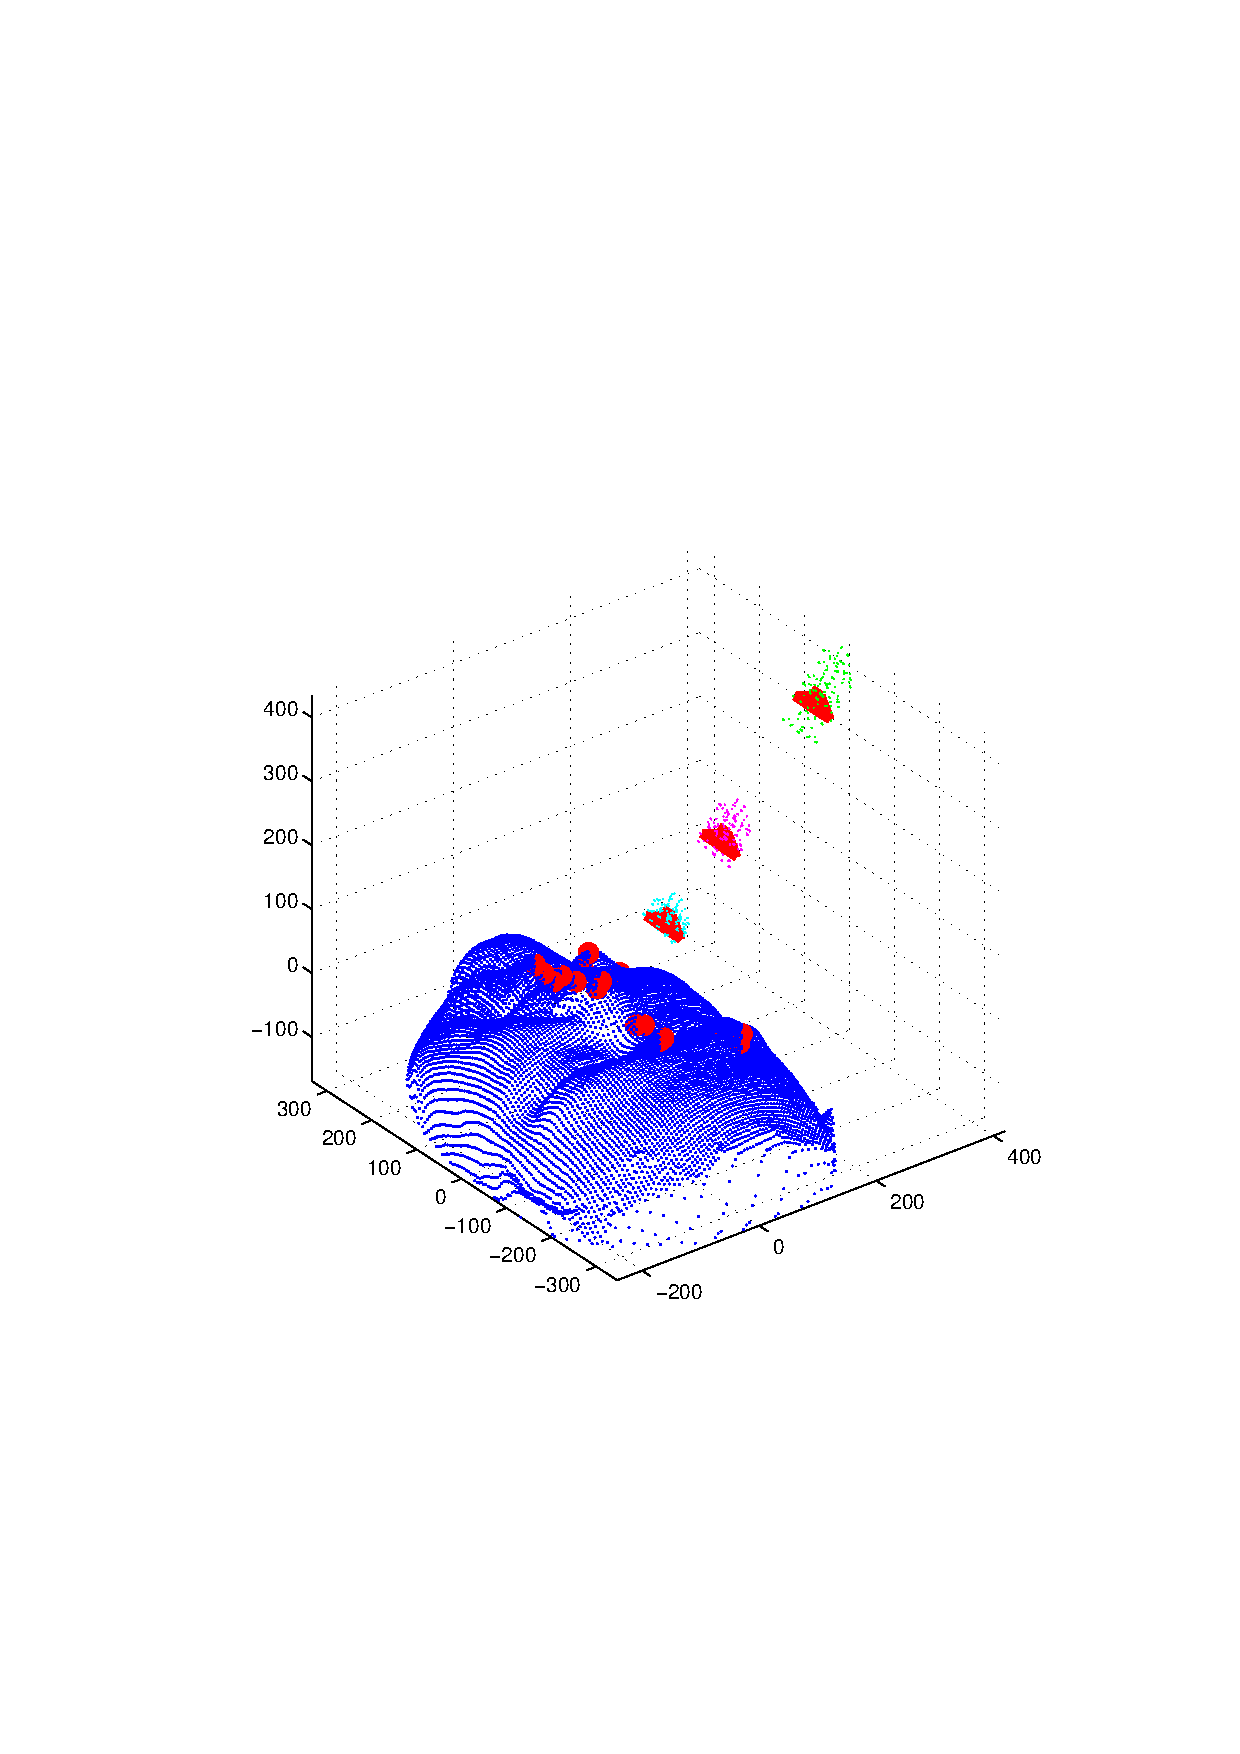
\includegraphics[width=.45\linewidth]{../resources/figures/cameraloc_3q.png} &
\includegraphics[width=.45\linewidth]{../resources/figures/errorbar_3q.png}
\end{tabular}
\end{figure}

\bibliographystyle{splncs}
\bibliography{library}

\end{document}
